% This document assumes the XeLaTeX engine
\documentclass[10pt]{article}

% ────────────────────────────────────────────────────────────────────────────
% Setup (Document Preamble)
% ────────────────────────────────────────────────────────────────────────────

% ─────────────────────────────────────────────
% Packages
% ─────────────────────────────────────────────
\usepackage{geometry}
\usepackage{fancyhdr}
\usepackage{xcolor}
\usepackage{hyperref}
\usepackage[most]{tcolorbox}
\usepackage{titlesec}
\usepackage{graphicx}
\usepackage{lipsum}

% Use Roboto font
\usepackage{fontspec}

% Bibliography
\usepackage[backend=biber,style=ieee,urldate=iso]{biblatex}
\addbibresource{references.bib}
\ExecuteBibliographyOptions{url=true,urldate=iso,seconds=true}

% Improve URL spacing in references
\usepackage{xurl}
\urlstyle{same}
\Urlmuskip=0mu

% Setup items for header/footer and page number
\geometry{margin=1in}
\pagestyle{fancy}
\fancyhf{} % clear header/footer
\fancyfoot[C]{\thepage} % centered page number
\renewcommand{\headrulewidth}{0pt}
\renewcommand{\footrulewidth}{0pt}

% Move footer up from the bottom margin to adjust page number down
\setlength{\footskip}{50pt}

\setmainfont{Roboto}[
  UprightFont    = *-Regular,
  ItalicFont     = *-Italic,
  BoldFont       = *-Bold,
  BoldItalicFont = *-BoldItalic,
]

\usepackage{newunicodechar}
\newunicodechar{→}{\ensuremath{\rightarrow}}

\usepackage{parskip}

% TikZ libs for diagrams
\usepackage{tikz}
\usetikzlibrary{arrows.meta,backgrounds,positioning,shapes.geometric,fit,calc}

% Relax the word wrapping (no aggressive hyphens)
\usepackage[none]{hyphenat}
\emergencystretch=2em

% Flag to distinguish title page vs the rest
\newif\ifGigaTitlePage
\GigaTitlePagetrue

\graphicspath{{image/}}

% For page bg watermarks
\AddToHook{shipout/background}{%
  \begin{tikzpicture}[remember picture,overlay]
    \ifGigaTitlePage
      % Title page: Smaller with higher opacity
      \node[
        anchor=center,
        opacity=1
      ] at (current page.center)
      {
        
\includegraphics[width=0.5\paperwidth]{logo_square.png}
      };
    \else
      % Other pages: Larger with less opacity
    %   \node[
    %     anchor=center,
    %     opacity=0.04
    %   ] at (current page.center)
    %   {
    %     
\includegraphics[width=1.1\paperwidth]{logo_square.png}
    %   };
    {} % Removed watermark from non-title page
    \fi
  \end{tikzpicture}%
}

% For tables
\usepackage{array}
\usepackage{tabularx}
\usepackage{booktabs}
\usepackage[table]{xcolor} % enables \rowcolor, \columncolor, \cellcolor

% Helps ensure figures remain in a section via FloatBarrier
\usepackage[section]{placeins}

% ─────────────────────────────────────────────
% GigaStar Brand Colors
% ─────────────────────────────────────────────

% Primary colors
\definecolor{GigaMint}{HTML}{00FAB9}
\definecolor{GigaRose}{HTML}{FF87D2}
\definecolor{GigaPeach}{HTML}{FA8282}
\definecolor{GigaIris}{HTML}{AAA0FF}
\definecolor{GigaLilac}{HTML}{7D5FFF}
\definecolor{GigaMov}{HTML}{B95FFF}
\definecolor{GigaIndigo}{HTML}{1641FF}
\definecolor{GigaElectro}{HTML}{14FAFF}

% Misc colors
\definecolor{GigaOffWhite}{HTML}{FAFAFA}
% \definecolor{GigaBlackTxt}{HTML}{17171D}
\definecolor{GigaBlackTxt}{HTML}{000000}
\definecolor{GigaGreyTxt}{HTML}{606060}
\definecolor{GigaDarkGrey}{HTML}{606060}
\definecolor{GigaLightGrey}{HTML}{A0A0A0}

% ─────────────────────────────────────────────
% Styling
% ─────────────────────────────────────────────

% Page background
\pagecolor{GigaOffWhite}

% Default text
\color{GigaBlackTxt}

% Remove colorbox padding
\setlength{\fboxsep}{0pt}

% GigaStar section with offset bg mint highlight - Mimics Website but look busy
% \newcommand{\GigaSection}[1]{%
%   \begin{tikzpicture}[baseline=(title.base)]
%     % Title text
%     \node[inner sep=0pt, anchor=west] (title)
%       {\Large#1};
%     % Background bar
%     \begin{scope}[on background layer]
%       \fill[GigaMint]
%         % Bottom-left corner:
%         %   - move right by 0.5em
%         %   - move up a bit (0.2ex) from the text baseline
%         ([xshift=0.5em,yshift=0.2ex]title.south west)
%         rectangle
%         % Top-right corner:
%         %   - move left by 0.5em
%         %   - bar height 1.6ex above the bottom
%         ([xshift=-0.5em,yshift=1.6ex]title.south east);
%     \end{scope}
%   \end{tikzpicture}%
% }

% GigaStar section background mint
% \newcommand{\GigaSection}[1]{%
%   \begin{tikzpicture}[baseline=(title.base)]
%     % Title text
%     \node[inner sep=0pt, anchor=west] (title)
%       {\Large#1};
%     % Background bar
%     \begin{scope}[on background layer]
%       \fill[GigaMint]
%         % Bottom-left corner:
%         ([xshift=-0.0em,yshift=-0.2ex]title.south west)
%         rectangle
%         % Top-right corner:
%         ([xshift=0.0em,yshift=2ex]title.south east);
%     \end{scope}
%   \end{tikzpicture}%
% }

% Section (H1)
% \titleformat{\section}
%   {}{}{0pt}{\GigaSection}
% \titlespacing*{\section}{0pt}{2.0em}{1.0em}

% Section (H1) — all caps, no number, no label spacing
\titleformat{\section}
  {\large\bfseries\color{GigaLilac}}
  {\thesection\quad}{0pt}{} % With number
%   {}{0pt}{\MakeUppercase} % Without number and ucase
\titlespacing*{\section}{0pt}{2.0em}{1.0em}

% Subsection (H2)
\titleformat{\subsection}
  {\normalsize\bfseries\color{GigaLilac}}
  {\thesubsection}{0.75em}{}
\titlespacing*{\subsection}{0pt}{1.5em}{0.75em}

% Subsubsection (H3)
\titleformat{\subsubsection}
  {\normalsize\bfseries\color{GigaMov}}
  {\thesubsubsection}{0.75em}{}
\titlespacing*{\subsubsection}{0pt}{1.0em}{0.5em}

% Hyperref Styles
\hypersetup{
  colorlinks=true,
  linkcolor=GigaIndigo,
  urlcolor=GigaIndigo,
  citecolor=GigaIndigo,
}

% Callout Box
\newtcolorbox{GsNoteLow}{
  colback=GigaLightGrey!10,
  colframe=GigaLightGrey,
  title=Minor Note,
  fonttitle=\bfseries,
}

% Callout Box
\newtcolorbox{GsNoteHigh}{
  colback=GigaRose!10,
  colframe=GigaRose,
  title=Important Note,
  fonttitle=\bfseries,
}

% Words to not hyphenate
\hyphenation{revenue}

% Simple "source citation" helper that links to Appendix items by label
\newcommand{\src}[1]{\textsuperscript{\hyperref[#1]{[\ref*{#1}]}}}

% ────────────────────────────────────────────────────────────────────────────
% Document
% ────────────────────────────────────────────────────────────────────────────
\begin{document}
\sloppy % Prevent aggressive wrapping

% ─────────────────────────────────────────────
% Document Title Page
% ─────────────────────────────────────────────
\begin{titlepage}
    \newgeometry{left=1in,right=1in,top=1.2in,bottom=1.2in}

    % Uncomment to see the color palette
    % \noindent\colorbox{GigaMint!90}{\parbox{\dimexpr\textwidth\relax}{\rule{0pt}{1.2cm}}}
    % \noindent\colorbox{GigaRose!90}{\parbox{\dimexpr\textwidth\relax}{\rule{0pt}{1.2cm}}}
    % \noindent\colorbox{GigaPeach!90}{\parbox{\dimexpr\textwidth\relax}{\rule{0pt}{1.2cm}}}
    % \noindent\colorbox{GigaIris!90}{\parbox{\dimexpr\textwidth\relax}{\rule{0pt}{1.2cm}}}
    % \noindent\colorbox{GigaLilac!90}{\parbox{\dimexpr\textwidth\relax}{\rule{0pt}{1.2cm}}}
    % \noindent\colorbox{GigaMov!90}{\parbox{\dimexpr\textwidth\relax}{\rule{0pt}{1.2cm}}}
    % \noindent\colorbox{GigaIndigo!90}{\parbox{\dimexpr\textwidth\relax}{\rule{0pt}{1.2cm}}}
    % \noindent\colorbox{GigaElectro!90}{\parbox{\dimexpr\textwidth\relax}{\rule{0pt}{1.2cm}}}

    % Top color bar
    \noindent\colorbox{GigaIris}{\parbox{\dimexpr\textwidth\relax}{\rule{0pt}{1.0cm}}}

    \vspace{0.7cm}

    % Logo (optional)
    \begin{center}
        %\includegraphics[width=0.35\linewidth]{images/gigastar-logo.png}

        % Title:
        {\Huge \color{GigaMov} \textbf{The Vault Contract Ecosystem}}

        % Subtitle:
        {\large \color{GigaMov}\textbf{for Revenue Distribution and Digital Asset Securities}}

        \vspace{0.5cm}

        {\large \color{GigaBlackTxt}\textbf{Technical Whitepaper}}

        % Technical Descriptor
        {\color{GigaBlackTxt}A Reconciliation-First Control Plane for Deterministic, Auditable Proposal Execution on EVM}

        % Logo centered
        % \begin{center}
        %     
\includegraphics[width=0.5\linewidth]{image/logo_square.png}
        % \end{center}
        % \vspace{1.1cm}

        \vspace{11.0cm}

        % Author
        {\large
            Jason Aubrey \\
            Co-Founder \& Chief Architect \\
            GigaStar Technologies, LLC
        }

        \vspace{0.5cm}

        % Document Status
        {\large v1.0-internal RFC}\break
        {\large January 1, 2026}

        \vspace{0.5cm}

    \end{center}

    \vfill

    % Bottom color bar
    \noindent\colorbox{GigaIris}{\parbox{\dimexpr\textwidth\relax}{\rule{0pt}{1.0cm}}}

    \restoregeometry
\end{titlepage}
\GigaTitlePagefalse % Set var to false

\newgeometry{left=0.75in,right=0.75in,top=1in,bottom=1.1in}
\tableofcontents
\newpage
\newgeometry{left=0.75in,right=0.75in,top=1in,bottom=0.5in}

% Reduce footer to adjust page number up
\setlength{\footskip}{12pt}

% ─────────────────────────────────────────────
% Document Content
% ─────────────────────────────────────────────

% ─────────────────────────────────────────────
\section{Abstract}
% ─────────────────────────────────────────────
This whitepaper presents the GigaStar Vault Ecosystem, a unified framework for digital-asset,
revenue-sharing securities designed to support growth in the Creator Economy. The system targets three
recurring event categories: issuance, recurring revenue, and secondary market trading. Each category
requires safe, auditable processes and a governance model intended to support compliance workflows,
safeguard Investors and Issuers, and preserve market integrity.

The Vault Ecosystem meets these requirements through a proposal-driven execution model on an
EVM-compatible blockchain. A governance kernel (the Vault) manages proposal lifecycle and voting, while
specialized manager contracts provide paged upload, cursor-based execution, and deterministic error
signaling. An application-level idempotency layer (CallTracker) enables deterministic retries for off-chain
automation under uncertain transaction outcomes. Public read surfaces and event-based telemetry
provide independent public auditability of key workflows and outcomes.

This paper focuses on the blockchain and adjacent components. It specifies the operational contract for
the Chain Sync service, describes the three primary workflows (instrument transfers, instrument revenues,
and revenue transfers), and documents the public audit surfaces.

% ─────────────────────────────────────────────
\section{Introduction}
% ─────────────────────────────────────────────
The Creator Economy continues to expand as Creators monetize digital work, generate recurring revenue,
and build financial relationships with their audiences. Small Creators seek capital to grow, large Creators
seek ways to diversify, while Fans and Investors seek regulated and transparent ways to participate.
Enabling these interactions at scale, safely, efficiently, and with clear auditability requires a structured
approach to revenue-sharing securities and their lifecycle operations.

GigaStar introduced a simple model \cite{chicago_innovation_awards_2025}: Creators sell a portion of their future revenue while Fans and Investors
buy or trade those revenue rights. The security represents a claim on future cash flows, not ownership of the
underlying digital asset itself. This distinction enables modular financing arrangements while preserving the
Creator's digital asset ownership and control.

From an engineering perspective, the core challenge is operational: issuance, recurring revenue allocation,
and transfer events must execute deterministically, remain verifiable under partial progress, and tolerate
real-world failure modes such as timeouts, retries, and gas-bounded execution. The Vault Ecosystem is
designed to provide these properties through on-chain governance, bounded execution, and a
reconciliation-first orchestration model.

% ──────────────────────
\subsection{History \& Motivation}
% ──────────────────────
GigaStar's legacy system was built during a period of uncertainty around market maturity, regulatory
expectations, technological direction, and a quick go-to-market strategy. Web3 offered a transparent ledger,
a distributed authorization layer, and a low-cost mechanism for distributing revenue to a global Investor base. These benefits had to be balanced against practical user constraints, including a heterogeneous population of existing Web3
users, newcomers with limited Web3 familiarity, and users preferring a Web2-centric experience.

The initial system was built on the Polygon proof-of-stake network using ERC-721 \cite{ethereum_erc721} to prioritize
both leading wallet compatibility and network user growth. This architecture enabled rapid onboarding
and early revenue distribution workflows, but it imposed long-term limitations around fungibility,
liquidity, and secondary trading mechanics. It also surfaced operational requirements unique to
recurring revenue distribution at scale, including stablecoin transitions and off-ramp constraints.

Despite these challenges, the early platform operated reliably through ecosystem-wide transitions,
including Circle's migration from USDC.e to native USDC \cite{circle_usdc}, and it delivered meaningful revenue distributions
to Investors surpassing \$1,000,000 \cite{gigastar_milestone_2025}. The Vault Ecosystem is a replacement architecture designed
to support secondary market trading, stronger governance, deterministic execution, and transparent
reporting. This new system will be deployed to Coinbase's \cite{coinbase_about} Base network \cite{base_network} for improvements to
regulatory alignment, Investor protections, and institutional concerns such as expected long-term network health.

% ─────────────────────────────────────────────
\section{System Overview}
% ─────────────────────────────────────────────

% ──────────────────────
\subsection{Hybrid Architecture}
% ──────────────────────
The Vault Ecosystem spans on-chain contracts and off-chain services. This
paper primarily focuses on on-chain components, with off-chain components
described where necessary to define inputs, outputs, and operational
workflows.

\begin{itemize}
    \item \textbf{On-Chain Layer}: EVM contracts responsible for securities
          issuance and ownership management, recurring revenue distributions,
          proposal-oriented governance, role-based access control, activity
          telemetry, Investor and Issuer safeguards, and upgradeability.

    \item \textbf{Off-Chain Layer}: External integrations, data pipelines,
          governance workflows, transaction coordinators, services for frontend,
          backend, and durable data storage.
\end{itemize}

\begin{GsNoteHigh}
    The system is on-chain where appropriate for governance, revenue management, and public transparency;
    off-chain where appropriate for integration with Web2 systems, and faster development cycles.
\end{GsNoteHigh}

% ──────────────────────
\subsection{Roles}
% ──────────────────────
The Vault Ecosystem is role-gated. The key roles are:

\begin{itemize}
    \item \textbf{Public}: Read-only observers (for auditing and transparency)
    \item \textbf{Agent}: Privileged automation for proposals (creating, uploading, sealing, and executing)
    \item \textbf{Voter}: Approves or rejects proposals by quorum
    \item \textbf{Admin}: Configuration and upgrade authority
\end{itemize}

% ──────────────────────
\subsection{Trust Boundaries}
% ──────────────────────
The system is designed around a clear trust boundary:

\begin{itemize}
    \item \textbf{Control-plane (off-chain)}: proposes and drives workflows.
          Transactions may experience uncertain outcomes (timeouts, dropped
          receipts, restarts) and therefore require deterministic retry and
          reconciliation.

    \item \textbf{Data-plane (on-chain)}: the authoritative state machine.
          Contracts enforce proposal lifecycle rules, role gating, upload integrity,
          bounded execution, and public auditability - in addition to attributes implicit
          to the underlying network such as a distributed ledger and cryptographic proofs.
\end{itemize}

% ──────────────────────
% Diagram: Control Plane vs On-chain
% ──────────────────────
\begin{figure}[h!]
    \centering
    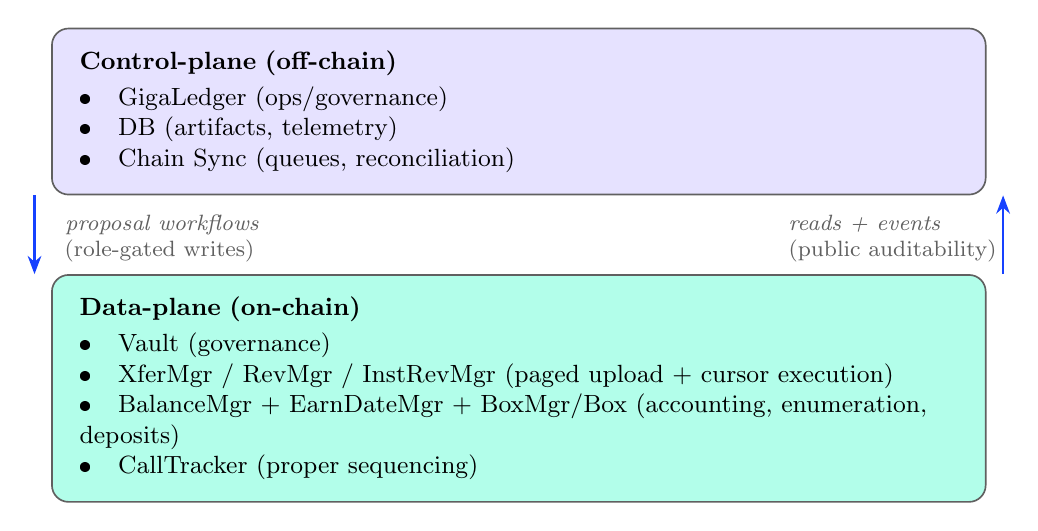
\begin{tikzpicture}[
            font=\small,
            >=Stealth,
            node distance=10mm,
            box/.style={
                    draw=GigaDarkGrey,
                    line width=0.6pt,
                    rounded corners=6pt,
                    inner xsep=10pt,
                    inner ysep=8pt,
                    align=left,
                    text width=0.92\textwidth
                },
            offchain/.style={box, fill=GigaIris!30},
            onchain/.style={box, fill=GigaMint!30},
            arrow/.style={-Stealth, thick, draw=GigaIndigo},
            alabel/.style={
                    text opacity=1,
                    inner sep=2pt,
                    font=\footnotesize\color{GigaGreyTxt},
                    align=left
                },
        ]

        % Boxes
        \node[offchain] (cp) {
            \textbf{Control-plane (off-chain)}\\[2pt]
            \textbullet \quad GigaLedger (ops/governance)\\
            \textbullet \quad DB (artifacts, telemetry)\\
            \textbullet \quad Chain Sync (queues, reconciliation)
        };

        \node[onchain, below=of cp] (dp) {
            \textbf{Data-plane (on-chain)}\\[2pt]
            \textbullet \quad Vault (governance)\\
            \textbullet \quad XferMgr / RevMgr / InstRevMgr (paged upload + cursor execution)\\
            \textbullet \quad BalanceMgr + EarnDateMgr + BoxMgr/Box (accounting, enumeration, deposits)\\
            \textbullet \quad CallTracker (proper sequencing)
        };

        % Arrows (use midpoints on edges to avoid corner hits)
        \draw[arrow]
        ([xshift=-6pt]cp.south west) -- ([xshift=-6pt]dp.north west)
        node[alabel, pos=0.55, right] {\textit{\quad proposal workflows}\\\quad (role-gated writes)};

        \draw[arrow]
        ([xshift=6pt]dp.north east) -- ([xshift=6pt]cp.south east)
        node[alabel, pos=0.45, left] {\textit{reads + events}\\(public auditability)};

    \end{tikzpicture}

    \caption{Reconciliation-first control-plane and the authoritative on-chain data-plane.}
    \label{fig:hybrid-architecture}
\end{figure}

% ─────────────────────────────────────────────
\section{Contract Architecture}
% ─────────────────────────────────────────────
The Vault Ecosystem is composed of EVM contracts deployed with cross-contract references, operating
as a mesh of services. The EIP-170 contract size constraint of 24 KiB influenced modular decomposition
for deployment and upgradeability.

% ──────────────────────
\subsection{Primary Contracts}
% ──────────────────────
\begin{itemize}
    \item \textbf{Vault}: Governance kernel providing proposal lifecycle, role tracking, and manager contract routing

    \item \textbf{Crt}: Channel Revenue Token (ERC-1155) supporting a scalable, fungible, security token
\end{itemize}

% ──────────────────────
\subsection{Manager Contracts}
% ──────────────────────
\begin{itemize}
    \item \textbf{XferMgr}: Instrument transfer proposals (native, ERC-20 \cite{ethereum_erc20}, ERC-1155 \cite{ethereum_erc1155})

    \item \textbf{RevMgr}: Revenue transfer proposals

    \item \textbf{InstRevMgr}: Instrument revenue proposals

    \item \textbf{BalanceMgr}: Tracks owner balances

    \item \textbf{EarnDateMgr}: Instrument and earn-date indexing

    \item \textbf{BoxMgr / Box}: Manages a deposit address per revenue stream for segregated audit trails
\end{itemize}

% ──────────────────────
\subsection{Reliability Substrate}
% ──────────────────────
\begin{itemize}
    \item \textbf{CallTracker}: Deterministic retries for off-chain callers via (caller, seqNum, reqId), replay acknowledgment, and call result persistence
\end{itemize}

% ──────────────────────
\subsection{Off-Chain Access}
% ──────────────────────
All contract state is publicly accessible via the blockchain ledger. It can be accessed from block explorers,
custom applications, GigaStar's Portfolio web application for Investors, or the internal GigaLedger
application for operations and governance. This state provides full transparency to interested parties.

During phases of issuance, trading, or revenue distribution, proposals are created by operations staff and
their actions provide inputs upstream of a privileged Agent automation role. Staff with Voter roles review
proposals via the GigaLedger and approve or reject them. Upon approval, backend services execute
proposals to change on-chain state, such as distributing revenue or transferring securities.

% ─────────────────────────────────────────────
\section{Design Principles}
% ─────────────────────────────────────────────
The Vault Ecosystem is organized around the following principles:

\begin{itemize}
    \item \textbf{Public Auditability}: Public view functions and events enable independent workflow verification

    \item \textbf{Multi-sig Proposals}: Proposals are gated by a voting quorum (ie multiple signatures)

    \item \textbf{Bounded Work}: Large payloads are uploaded in pages for gas-bounded progress; execution is cursor-based to guarantee resumability

    \item \textbf{Determinism by Protocol}: Uncertain outcomes due to a failure in request/response pipelines are handled by a protocol of reliability mechanisms that resolve to a certain outcome (eg replay-safe requests, idempotency, request identifiers, sequence numbers, cached results, replayable events)
\end{itemize}

\clearpage
% ─────────────────────────────────────────────
\section{Design Rationale \& Alternatives}
% ─────────────────────────────────────────────

% ──────────────────────
\subsection{Proposal-Driven Governance}
% ──────────────────────
Proposal-driven governance provides a verifiable control surface for high-impact state transitions
(issuance, revenue allocation, and transfers). The intent is to make every material change:
\begin{itemize}
    \item Explicitly authorized (quorum-voted)
    \item Replayable and resumable under gas limits
    \item Independently auditable by public observers (full-transparency)
\end{itemize}

\textbf{Alternative: Single-signer actions.}
A single-signer model directly executes state mutations without a transparent quorum. While simpler, it reduces audit structure, complicates post-incident attribution, and increases blast radius under key compromise.

% ──────────────────────
\subsection{Paged Upload and Sealing}
% ──────────────────────
Operational payloads can be large (eg many transfers, many owners, many earn-date allocations). Uploading in pages enforces a bounded per-transaction cost and allows robust retries. Sealing makes the payload immutable so that governance decisions can refer to a stable artifact.

\textbf{Alternative: Single-transaction upload.} A single upload transaction is simpler but fails for many realistic batch sizes under EVM gas constraints. Pages also amortize gas fees and processing time by grouping line items into a single transaction.

\textbf{Alternative: Off-chain payloads only.} On-chain payloads allow a proposal request to be independently verified via Web3 methods and improve auditability due to the inherent immutability and distributed nature of the underlying ledger.

% ──────────────────────
\subsection{Cursor-Based Execution}
% ──────────────────────
Execution is modeled as a resumable state machine. Cursors provide monotonic progress and deterministic retry under partial completion and out-of-gas conditions.

\textbf{Alternative: Execute-all-or-revert.} Transaction gas bounds do not yet support the required throughput for
most proposals. Sharding proposal payloads to fit gas bounds reinvents proposals with less elegance.

% ──────────────────────
\subsection{Modular Manager Contracts}
% ──────────────────────
EIP-170 contract-size constraints materially influence implementation which would otherwise require a dynamic library that would have a competing set of complexities and constraints. Separating proposal types across managers focuses each contract on a smaller set of invariants and provides logical and organizational boundaries for logic and data.

\textbf{Alternative: Monolithic manager.} A monolithic contract with a dynamic library can reduce cross-contract hops but increases upgrade risk, auditing complexity, and size-limit pressure.

% ──────────────────────
\subsection{CallTracker Exists On-Chain}
% ──────────────────────
CallTracker addresses a real-world integration gap: off-chain automation operates under uncertain transaction outcomes (eg stale nodes, timeouts, network flaps, process restarts). By making retry semantics explicit on-chain via (\texttt{caller, seqNum, reqId}), the protocol becomes deterministic even when the network is not (inspired by ARPANET-era reliability \cite{rfc_793} \cite{rfc_9293}).

\textbf{Alternative: Purely off-chain idempotency.} Purely off-chain idempotency fails under ambiguous “did it execute?” conditions. For example, pre-calculating a transaction hash before submission could in theory allow the transaction status to be known under uncertain conditions but due to nuances of latency and stale nodes, a false negative could occur leading to a request replay and duplicate action. CallTracker avoids this scenario via a first-class signal for determinism-by-protocol and on-chain idempotency.

% ──────────────────────
\subsection{Explicit Public Audit Surfaces}
% ──────────────────────
While many systems may use public read functions and events as simply "debug output", this system considers these to be a product surface for Investors, regulators, counterparties, and internal operations. The goal is to make key workflows publicly verifiable without privileged access for full-transparency.

\textbf{Alternative: Explorer-only visibility.} Block explorers provide potential transparency but their utility is often limited or disabled without a proper public audit surface.

% ─────────────────────────────────────────────
\section{Securities}
% ─────────────────────────────────────────────

% ──────────────────────
\subsection{Securitization}
% ──────────────────────
In this paper, an instrument is a revenue sharing security aligned with the SEC's Reg CF \cite{finra_funding_portals};
as such, protocols are designed to support compliance controls which safeguard Investors and Issuers.

% ──────────────────────
\subsection{Instrument Lifecycle}
% ──────────────────────
An instrument progresses through phases of the following lifecycle:

\begin{center}
    \color{GigaIndigo}Issuance → Holding Period → Roll/Conversion → Trading
\end{center}

After Issuance, revenue is distributed based on the terms of the security/instrument - extending from the holding period through the trading phase.

Issuance is followed by a Reg CF mandated Investor holding period (ie the instrument is not tradable). After this period, ownership in the non-tradable instrument is converted into ownership of a tradable instrument. The tradable instrument may contain units from multiple issuances, each of which are converted to equivalent fungible units.

For example over a period of time, a Creator may have 3 issuances (ABC.1, ABC.2, ABC.3) and each instrument eventually rolls into ABC.0 - a pool of fungible ABC revenue sharing units (RSUs). The roll may include a conversion to split/merge shares to create equivalent revenue sharing rates/percentages.

% ─────────────────────────────────────────────
\section{Definitions and Notation}
% ─────────────────────────────────────────────

This section defines recurring terms used normatively throughout this paper.

\subsection{Actors and Roles}
\begin{itemize}
    \item \textbf{Creator}: A monetized content creator who may become an Issuer of revenue shares via GigaStar.
    \item \textbf{Investor}: A revenue share owner via either the primary or secondary market.
    \item \textbf{Public}: Any observer with read-only access to on-chain state and events for transparency and auditability.
    \item \textbf{Agent}: A privileged automation role responsible for proposing, uploading, sealing, and executing workflows.
    \item \textbf{Voter}: An authorized role that approves or rejects proposals by quorum.
    \item \textbf{Admin}: A privileged role for configuration changes and upgrades.
\end{itemize}

\subsection{Proposal Terms}
\begin{itemize}
    \item \textbf{Proposal}: A governance-gated request to transition on-chain state using a structured payload and lifecycle.
    \item \textbf{Paged Upload}: Payload ingestion via multiple transactions, each bounded by gas limits.
    \item \textbf{Seal}: A lifecycle transition that makes a proposal payload immutable for governance review and execution.
    \item \textbf{Cursor-Based Execution}: Resumable execution where each call advances a stored cursor until completion.
    \item \textbf{Terminal Status}: A final proposal state after which no further state mutations occur for the proposal.
\end{itemize}

\subsection{Reliability and Sequencing}
\begin{itemize}
    \item \textbf{Retry Key}: The tuple \texttt{(caller, seqNum, reqId)} used to make on-chain outcomes deterministic under retries.
    \item \textbf{caller}: The address submitting a state-mutating transaction (typically an Agent).
    \item \textbf{seqNum}: A per-(contract, caller) monotonically increasing sequence number enforcing FIFO ordered writes.
    \item \textbf{reqId}: A request identifier (UUID) used to uniquely identify the intended operation under replay.
    \item \textbf{Replay}: A resubmitted request that behaves idempotently with respect to the original compact result.
    \item \textbf{Reconciliation}: The process of recovering correct state by querying authoritative on-chain state and (when required) replaying prior events.
\end{itemize}

\subsection{Normative Language}
The keywords \textbf{MUST}, \textbf{MUST NOT}, \textbf{SHOULD}, and \textbf{MAY} are to be interpreted as described in RFC 2119 \cite{rfc_2119}.

% ─────────────────────────────────────────────
\section{Core Invariants}
% ─────────────────────────────────────────────

This section lists system invariants treated as normative correctness conditions. They serve as a checklist for audits, reviews, and future refactors.

% ──────────────────────
\subsection{Governance and Status Invariants}
% ──────────────────────
\begin{itemize}
    \item \textbf{\texttt{I1} (Role-gated writes)}: All state-mutating operations are restricted to appropriate roles (Agent/Voter/Admin), with Public limited to read surfaces.

    \item \textbf{\texttt{I2} (Monotonic proposal status)}: Proposal status is monotonic; proposals cannot transition from a terminal state back into an active state.

    \item \textbf{\texttt{I3} (Payload immutability after seal)}: Once a proposal is sealed, its payload and relevant headers are immutable; governance decisions apply to a stable artifact.
\end{itemize}

% ──────────────────────
\subsection{Upload and Execution Invariants}
% ──────────────────────
\begin{itemize}
    \item \textbf{\texttt{I4} (Append-index correctness)}: Paged upload enforces strict append indexing via \texttt{iAppend} and \texttt{total}. Missing or duplicate pages are rejected deterministically.

    \item \textbf{\texttt{I5} (Cursor monotonicity)}: Execution cursors only move forward. If a proposal's status is terminal (eg Executed) then a request replay must not advance the proposal state.

    \item \textbf{\texttt{I6} (Bounded progress)}: Each execute call performs bounded work and returns typed progress, enabling resumption without requiring unbounded gas.
\end{itemize}

% ──────────────────────
\subsection{Accounting and Transfer Invariants}
% ──────────────────────
\begin{itemize}
    \item \textbf{\texttt{I7} (Conservation / consistency)}: Token transfers and balance mutations preserve defined conservation rules (eg instrument supply, per-source balance constraints, or accounting totals).

    \item \textbf{\texttt{I8} (Allocation sums)}: For instrument revenue, per-owner allocations must reconcile to the per-(instrument, earn date) totals within defined rounding rules.

    \item \textbf{\texttt{I9} (No duplicate effects under retry)}: Under the CallTracker protocol, at most one state-changing call can be accepted for a given (\texttt{caller, seqNum}); replays return the original result with a block number to retrieve related events from the historical ledger.
\end{itemize}

% ──────────────────────
\subsection{Auditability Invariants}
% ──────────────────────
\begin{itemize}
    \item \textbf{\texttt{I10} (Public verifiability)}: For each proposal workflow, sufficient public on-chain read surfaces and events exist to independently verify: proposal payload, lifecycle status, both proximate and terminal outcomes.
\end{itemize}

\clearpage
% ─────────────────────────────────────────────
\section{Proposal Model \& Lifecycle}
% ─────────────────────────────────────────────

% ──────────────────────
\subsection{Proposal Types}
% ──────────────────────
The primary proposal types covered in this paper are:

\begin{itemize}
    \item \textbf{Instrument Revenue} (\texttt{PropType.InstRev}): Instrument related Investor revenue tracking
    \item \textbf{Token Transfers} (\texttt{PropType.Xfer})
          \begin{itemize}
              \item \textbf{Instrument Transfers}: Ownership changes from issuance or trades
              \item \textbf{Revenue Transfers}: Revenue sharing payments to Investors
          \end{itemize}
\end{itemize}

% ──────────────────────
\subsection{Proposal Lifecycle By Role}
% ──────────────────────

% ──────────────────────
% Diagram: Lifecycle flow by Role
% ──────────────────────
\begin{figure}[h!]
    \centering
    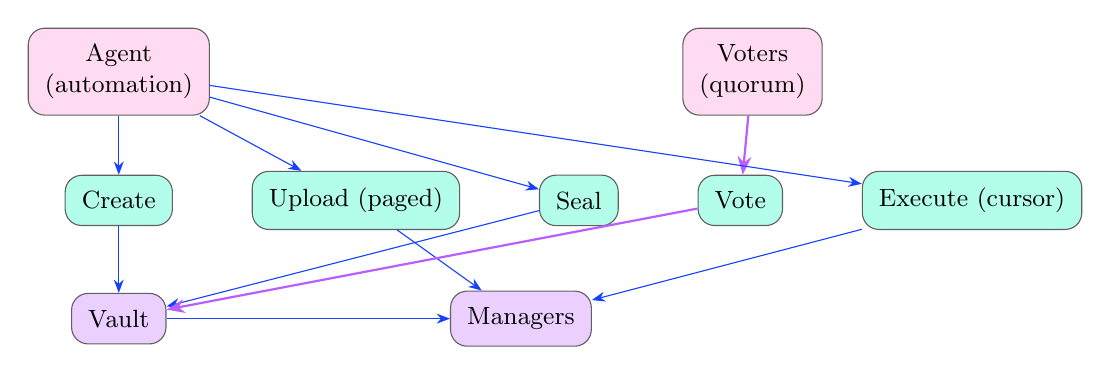
\begin{tikzpicture}[
            font=\small,
            actor/.style={draw=GigaDarkGrey, rounded corners=6pt, fill=GigaRose!30, inner sep=6pt, align=center},
            wfstep/.style={draw=GigaDarkGrey, rounded corners=6pt, fill=GigaMint!30, inner sep=6pt, align=center},
            evm/.style={draw=GigaDarkGrey, rounded corners=6pt, fill=GigaMov!30, inner sep=6pt, align=center},
            arrow/.style={-Stealth, thin, draw=GigaIndigo},
            arrow2/.style={-Stealth, thick, draw=GigaMov},
        ]
        \node[actor] (agent) {Agent\\(automation)};
        \node[evm, below=2.25cm of agent] (vault) {Vault};
        \node[evm, right=3.6cm of vault] (mgr) {Managers};
        \node[actor, right=6cm of agent] (voter) {Voters\\(quorum)};

        \node[wfstep, below=0.75cm of agent] (s1) {Create};
        \node[wfstep, right=of s1] (s2) {Upload (paged)};
        \node[wfstep, right=of s2] (s3) {Seal};
        \node[wfstep, right=of s3] (s4) {Vote};
        \node[wfstep, right=of s4] (s5) {Execute (cursor)};

        \draw[arrow] (agent) -- (s1);
        \draw[arrow] (s1) -- node[left]{} (vault);
        \draw[arrow] (vault) -- node[below]{} (mgr);

        \draw[arrow] (agent) -- (s2);
        \draw[arrow] (s2) -- node[right]{} (mgr);

        \draw[arrow] (agent) -- (s3);
        \draw[arrow] (s3) -- node[left]{} (vault);

        \draw[arrow2] (voter) -- (s4);
        \draw[arrow2] (s4) -- node[below left]{} (vault);

        \draw[arrow] (agent) -- (s5);
        \draw[arrow] (s5) -- node[right]{} (mgr);
    \end{tikzpicture}
    \caption{Role-oriented proposal workflow}
    \label{fig:proposal-seq-role}
\end{figure}

GigaLedger uses crypto-signing for request authenticity, authentication, authorization, and attribution:
\begin{itemize}
    \item \textbf{Proposal Request}: Each proposal request is signed similar to a Web3 tunnel through the Web2 stack.

    \item \textbf{Proposal Voting}: Votes are cast via off-chain signing (EIP-712 \cite{eip_712}) and relayed to the EVM to centralize on-chain concerns (gas, connectivity, etc). Vault also supports direct on-chain signing.
\end{itemize}

% ──────────────────────
\subsection{Proposal Lifecycle By Status}
% ──────────────────────
A proposal generally transits from status \texttt{Pending} to \texttt{Executed} but may deviate to another terminal state.

% Status colors
\definecolor{GigaTermOrange}{HTML}{C05A00} % dark-ish orange, prints well
\definecolor{GigaTermGreen}{HTML}{0B5D1E}  % dark green, prints well

\newcommand{\NodeGood}[1]{{\textcolor{GigaTermGreen}{#1}}}
\newcommand{\NodeFatal}[1]{\textcolor{GigaTermOrange}{#1}}

% ──────────────────────
% Diagram: Lifecycle flow by Status
% ──────────────────────
\begin{figure}[h!]
    \centering
    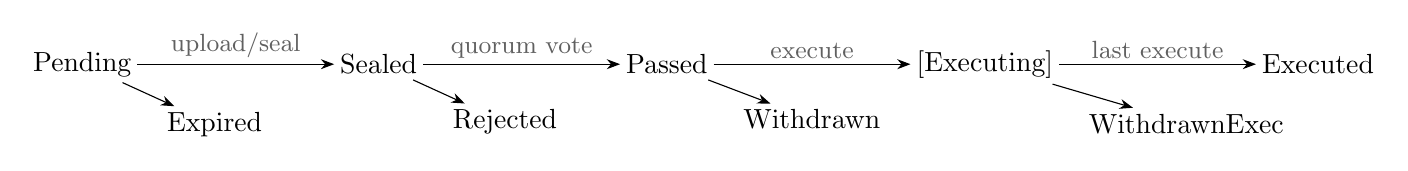
\begin{tikzpicture}[
            font=\normalsize,
            >=Stealth,
            node distance=2.5cm,
            main/.style={inner sep=2pt, align=center},
            term/.style={inner sep=2pt, align=center},
        ]

        % Main line
        \node[main] (pending)                   {\NodeGood{Pending}};
        \node[main, right=of pending] (sealed)  {\NodeGood{Sealed}};
        \node[main, right=of sealed]  (passed)  {\NodeGood{Passed}};
        \node[main, right=of passed]  (execing) {\NodeGood{[Executing]}};
        \node[main, right=of execing] (execed)  {\NodeGood{Executed}};

        % Transitions on main line (with labels)
        \draw[->] (pending) -- node[
            midway,
            above,
            inner sep=2pt,
            font=\small\color{GigaGreyTxt}
        ] {upload/seal} (sealed);

        \draw[->] (sealed) -- node[
            midway,
            above,
            inner sep=2pt,
            font=\small\color{GigaGreyTxt}
        ] {quorum vote} (passed);

        \draw[->] (passed) -- node[
            midway,
            above,
            inner sep=2pt,
            font=\small\color{GigaGreyTxt}
        ] {execute} (execing);

        \draw[->] (execing) -- node[
            midway,
            above,
            inner sep=2pt,
            font=\small\color{GigaGreyTxt}
        ] {last execute} (execed);

        % Terminal/side statuses (offset below)
        \node[term, below right=0.3cm and 0.3cm of pending] (expired){\NodeFatal{Expired}};
        \node[term, below right=0.3cm and 0.3cm of sealed] (rejected){\NodeFatal{Rejected}};
        \node[term, below right=0.3cm and 0.3cm of passed] (withdrawn){\NodeFatal{Withdrawn}};
        \node[term, below right=0.3cm and 0.3cm of execing] (withdrawnExec){\NodeFatal{WithdrawnExec}};

        % Diagonal arrows down
        \draw[->] (pending) -- (expired);
        \draw[->] (sealed)  -- (rejected);
        \draw[->] (passed)  -- (withdrawn);
        \draw[->] (execing) -- (withdrawnExec);

    \end{tikzpicture}
    \caption{Status-oriented proposal workflow}
    \label{fig:proposal-seq-status}
\end{figure}

The status model is explicitly partitioned to allow consumers to treat a proposal as terminal without enumerating every terminal reason.

% ──────────────────────
\subsection{Manager Patterns}
% ──────────────────────
Manager contracts implement two recurring patterns:

\begin{itemize}
    \item \textbf{Paged Upload}: Strict append-indexing using \texttt{iAppend}
          and \texttt{total} for deterministic payload ingestion

    \item \textbf{Execution Cursor}: Stored cursors enable proposal progress and resumption, with typed return codes for progress and completion
\end{itemize}

\clearpage
% ─────────────────────────────────────────────
\section{Primary Workflows}
% ─────────────────────────────────────────────

The following workflows contain various checks and simulations to fail fast where practical. However, proper sequencing is assumed to reduce algorithmic complexity and ensure prerequisite state exists per proposal. Core behaviors are delegated from Vault to manager contracts. Multiple instruments are supported per proposal.

% ──────────────────────
\subsection{Workflow A: Instrument Transfer}
% ──────────────────────
\textbf{Prerequisites}: Off-chain actions necessitate instrument transfers (eg issuance or trades). An issuance respects the security terms and a trade respects the outstanding instrument supply.

This workflow supports multiple instrument transfers and the proposal sequence:

\begin{itemize}
    \item \textbf{Create}: Agent creates a transfer proposal in Vault
    \item \textbf{Upload}: Agent uploads the proposal payload via pages of lines (ie transfer details)
    \item \textbf{Seal}: Agent seals proposal
    \item \textbf{Vote}: Voters approve or reject the proposal via a quorum of \texttt{Vote.Yay} or \texttt{Vote.Nay}
    \item \textbf{Execute}: Agent executes via Vault; Vault delegates to XferMgr until completion
\end{itemize}

\begin{GsNoteLow}
    Transfers of native coin (eg ETH) and other tokens (ERC-20 and ERC-1155 \cite{ethereum_erc1155}) are also supported to handle edge-cases such as reversing incorrect upstream deposits that would otherwise be permanently locked/lost.
\end{GsNoteLow}

% ──────────────────────
\subsection{Workflow B: Instrument Revenue}
% ──────────────────────
\textbf{Prerequisite}: Instrument revenue was not previously allocated for the given key (instrument, earn date). The ownership snapshot per key is valid and complete with respect to the outstanding instrument supply.

This workflow allocates revenue per Instrument and per related Investors for an earn date via the proposal sequence:

\begin{itemize}
    \item \textbf{Create}: Agent creates an InstRev proposal in Vault
    \item \textbf{Upload InstRev}: Agent uploads instrument revenue lines in pages
    \item \textbf{Upload Owners}: Agent uploads ownership snapshots per key (instrument, earn date)
    \item \textbf{Seal}: Agent seals proposal
    \item \textbf{Vote}: Voters approve or reject the proposal via a quorum of \texttt{Vote.Yay} or \texttt{Vote.Nay}
    \item \textbf{Execute}: Agent executes via Vault; Vault delegates to InstRevMgr until completion
\end{itemize}

\begin{GsNoteLow}
    If instrument revenue was previously allocated for the given key then it is considered an adjustment. Adjustments are non-destructive as they append to the ledger history so the full audit-trail is available for public observation (ie full transparency).
\end{GsNoteLow}

% ──────────────────────
\subsection{Workflow C: Revenue Transfer / Distributions (RevDist)}
% ──────────────────────
Revenue distributions are modeled as transfer proposals with a revenue-distribution flag. This mode
is constrained to ERC-20 (due to contract size limitations), and it commonly follows
the execution logic of an InstRev proposal with Vault delegation to RevMgr.

A key safety property in RevDist mode is a per-source running balance simulation anchored from
BalanceMgr, which reduces the likelihood of executing underfunded batches and provides deterministic
failure modes when inputs are inconsistent. This provides an extra layer of safety against upstream
protocol violations which should not happen (ie resiliency/anti-fragility via expecting the unexpected).

\clearpage
% ─────────────────────────────────────────────
\section{Reliability Substrate: CallTracker Contract}
% ─────────────────────────────────────────────

% ──────────────────────
\subsection{Uncertain Outcomes and Retries}
% ──────────────────────
Automation driving on-chain writes must tolerate uncertain outcomes inherent to unreliable mechanisms such as
RPC connections, mempool protocols, and process restarts. Correctness requires determinism manifest from
multiple layers of reliability mechanisms.

An off-chain call may be inconsistent with on-chain state in multiple ways such as a bad sequence number (too low or high) or a duplicate request. While conflicts are off the "happy-path" of standard interactions, each is expected
as they must be mitigated rather than solved such that the on-chain state prevails as the source-of-truth and the off-chain client must recover via a reconciliation protocol.

% ──────────────────────
\subsection{Deterministic Retry Key}
% ──────────────────────
CallTracker provides deterministic retry semantics keyed by:

\begin{itemize}
    \item \textbf{reqId}: Request identifier (UUID)
    \item \textbf{caller}: Address submitting requests (eg An Agent)
    \item \textbf{seqNum}: Expected sequence number (monotonic)
\end{itemize}

% ──────────────────────
\subsection{Deterministic Replay}
% ──────────────────────

If a call is replayed with the same key, the system sets a replay flag and returns a compact result tuple for recovery and reconciliation:

\begin{itemize}
    \item \textbf{reqId}: Request identifier (UUID)
    \item \textbf{rc}: Call return code, often relates to status/progress
    \item \textbf{lrc}: Line return code, often relates to a line/item
    \item \textbf{count}: Item count, often relates to items processed
    \item \textbf{blockNum}: For replay to find the original transaction
\end{itemize}

\begin{GsNoteHigh}
    Due to the distributed nature of blockchain nodes and state-synchronization latency, a contract's external view function call result may be stale; consequently, the most reliable recovery mechanism is to query the prior block via the \texttt{blockNum} to replay events from the transaction log.
\end{GsNoteHigh}

\clearpage
% ──────────────────────
\subsection{CallTracker Sequencing}
% ──────────────────────
While actions on-chain always have certain outcome after finality and/or sufficient confirms. CallTracker must provide certainty via determinism-by-protocol by treating replay as a first-class protocol action.

% ──────────────────────
% Diagram: Calltracker logic
% ──────────────────────
\begin{figure}[h!]
    \centering
    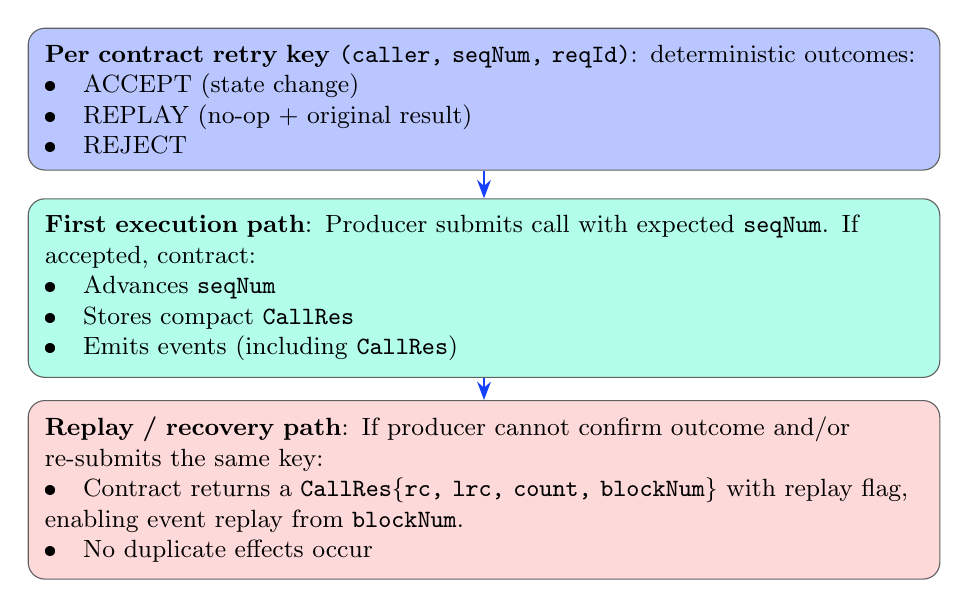
\begin{tikzpicture}[
            font=\small,
            box/.style={
                    draw=GigaDarkGrey,
                    rounded corners=6pt,
                    inner sep=6pt,
                    align=left,
                    text width=0.92\textwidth,  % key change: constrain text,
                    fill=GigaIndigo!30
                },
            ok/.style={box, fill=GigaMint!30},
            warn/.style={box, fill=GigaPeach!30},
            arrow/.style={-Stealth, thick, draw=GigaIndigo},
        ]

        \node[box] (key) {
            \textbf{Per contract retry key} \texttt{(caller, seqNum, reqId)}: deterministic outcomes:\\
            \textbullet \quad ACCEPT (state change) \\
            \textbullet \quad REPLAY (no-op + original result) \\
            \textbullet \quad REJECT
        };

        \node[ok, below=10pt of key] (first) {
            \textbf{First execution path}: Producer submits call with expected \texttt{seqNum}. If accepted, contract:\\
            \textbullet \quad Advances \texttt{seqNum}\\
            \textbullet \quad Stores compact \texttt{CallRes}\\
            \textbullet \quad Emits events (including \texttt{CallRes})
        };

        \node[warn, below=8pt of first] (replay) {
            \textbf{Replay / recovery path}: If producer cannot confirm outcome and/or re-submits the same key:\\

            \textbullet \quad Contract returns a \texttt{CallRes\{rc, lrc, count, blockNum\}} with replay flag, enabling event replay from \texttt{blockNum}.\\

            \textbullet \quad No duplicate effects occur
        };

        \draw[arrow] (key) -- (first);
        \draw[arrow] (first) -- (replay);

    \end{tikzpicture}
    \caption{CallTracker sequencing.}
    \label{fig:calltracker-determinism}
\end{figure}

This matrix defines the normative action taken by CallTracker under the cross-product of (seqNum relative to expect, reqId reuse, allow flag). It is intended to be read as a total function over request inputs.

\begin{figure}[h!]
    \centering
    \renewcommand{\arraystretch}{1.15}
    \setlength{\tabcolsep}{6pt}

    % Action row tints
    \newcommand{\RowAccept}{\rowcolor{GigaMint!30}}
    \newcommand{\RowReplay}{\rowcolor{GigaIndigo!30}}
    \newcommand{\RowReject}{\rowcolor{GigaPeach!30}}
    \newcommand{\RowInvalid}{\rowcolor{GigaLightGrey!30}}

    \begin{tabularx}{\textwidth}{
        c
        >{\raggedright\arraybackslash}p{2.0cm}
        >{\raggedright\arraybackslash}p{1.2cm}
        >{\raggedright\arraybackslash}p{1.2cm}
        >{\columncolor{GigaIndigo!6}\raggedright\arraybackslash}p{1.8cm} % Outcome: Action (tinted)
        >{\columncolor{GigaIndigo!6}\raggedright\arraybackslash}X        % Outcome: Description (tinted)
        }
        \toprule

        % Group header row
        \rowcolor{GigaLightGrey!30}
        \textbf{ }                                         &
        \multicolumn{3}{c}{\textbf{Request Input Factors}} &
        \multicolumn{2}{c}{\textbf{Outcome}}                                                                                                        \\
        \cmidrule(lr){2-4}\cmidrule(lr){5-6}

        % Column header row
        \rowcolor{GigaLightGrey!30}
        \textbf{Case}                                      &
        \textbf{SeqNum}                                    &
        \textbf{ReqId}                                     &
        \textbf{Allow}                                     &
        \textbf{Action}                                    &
        \textbf{Description}                                                                                                                        \\
        \midrule

        \RowReject
        \texttt{000}                                       & $< \text{expect}$ & New   & N/A & REJECT  & Stale seqNum with new reqId (invalid)      \\

        \RowReplay
        \texttt{011}                                       & $< \text{expect}$ & Reuse & Yes & REPLAY  & Replay prior req, same (caller, seqNum)    \\

        \RowReject
        \texttt{012}                                       & $< \text{expect}$ & Reuse & No  & REJECT  & Invalid replay, different (caller, seqNum) \\

        \RowAccept
        \texttt{100}                                       & $= \text{expect}$ & New   & N/A & ACCEPT  & Valid next FIFO request, state change      \\

        \RowInvalid
        \texttt{111}                                       & $= \text{expect}$ & Reuse & Yes & INVALID & Unreachable (curr seq can’t match prior)   \\

        \RowReject
        \texttt{112}                                       & $= \text{expect}$ & Reuse & No  & REJECT  & Invalid replay, mismatched seqNum          \\

        \RowReject
        \texttt{200}                                       & $> \text{expect}$ & New   & N/A & REJECT  & Future seqNum (FIFO violation)             \\

        \RowInvalid
        \texttt{211}                                       & $> \text{expect}$ & Reuse & Yes & INVALID & Unreachable (future seq can’t match prior) \\

        \RowReject
        \texttt{212}                                       & $> \text{expect}$ & Reuse & No  & REJECT  & Future seqNum (FIFO violation)             \\

        \bottomrule
    \end{tabularx}

    \caption{CallTracker request decision matrix for (caller, seqNum, reqId) reconciliation.}
    \label{tab:calltracker-matrix}
\end{figure}

Column descriptions:
\begin{itemize}
    \item \textbf{Case} Factor-coded case ID (mixed-radix) over the cartesian product enumeration
    \item \textbf{SeqNum} Each (\texttt{caller, reqId}) uniquely maps to one \texttt{seqNum}; possible values (<, ==, >)
    \item \textbf{ReqId} Each (\texttt{caller, seqNum}) uniquely maps to one \texttt{reqId}; possible values (New, Reuse)
    \item \textbf{Allow} (Allow `reqId` reuse), "Yes": prior call had the same (\texttt{caller, seqNum, reqId}); "No": \texttt{reqId} must be new; possible values (N/A, Yes, No)
\end{itemize}

A \texttt{seqNum} must increase monotonically per caller (FIFO) for a write to occur otherwise it is a replay or error.
Reuse never advances a \texttt{seqNum} as it is always either idempotent (replay) or an error.

\clearpage
% ─────────────────────────────────────────────
\section{Request Producers: Interface Contract}
% ─────────────────────────────────────────────
This section defines the normative contract for off-chain request producers (eg a Chain Sync service) that drives proposals. This control-plane must be deterministic and reconciliation-first.

% ──────────────────────
\subsection{Queue Discipline}
% ──────────────────────
Request producers should ensure requests are executed in FIFO order:
\begin{itemize}
    \item Implies each proposal should only be voted on after prior ones are approved or final
    \item Exceptions may exist for unrelated proposals, but consistently FIFO simplifies correctness
\end{itemize}

Each off-chain request/proposal contains an UUID identifier (\texttt{reqId}) and every contract write call in the proposal workflow sequence has an identifier that is a deterministic descendant of the proposal's \texttt{reqId}.

Each off-chain queue must be serviced by exactly one on/off-chain agent to preserve FIFO ordering, and:
\begin{itemize}
    \item Throughput can be increased by segmenting unrelated requests into separate queues
    \item More than one agent per queue risks race conditions and replay errors
    \item A single agent can manage multiple queues, but this may not justify the increased complexity
\end{itemize}

% ──────────────────────
\subsection{Concurrency Model (Control-Plane)}
% ──────────────────────
A \textbf{thread} is defined as a FIFO-ordered stream of state-mutating calls that share a sequence domain.
In the Vault Ecosystem, the primary sequence domain is \textbf{per contract, per caller}:
each contract maintains a monotonic \texttt{seqNum} for each caller address.

\textbf{Implication 1: Per-contract sequencing.}
In the short-term (eg during a process session), a request producer must track \texttt{seqNum} independently for each contract it writes to (eg Vault, XferMgr, RevMgr, etc). Two calls with the same \texttt{caller} sent to different contracts occupy different sequence domains and therefore have independent ordering constraints. In the long-term (eg between sessions - minutes later), on-chain state can be considered reliable to simplify away the need for off-chain state durability.

\textbf{Implication 2: Single-writer per thread.}
For correctness and simplicity, each (contract, caller) thread should have exactly one active writer at a time. Multiple writers increase the probability of replay/sequence conflicts and can degrade operational determinism.

\textbf{Implication 3: Parallelism via sharding.}
Throughput can be increased safely by sharding work across:
\begin{itemize}
    \item distinct contracts (eg XferMgr vs InstRevMgr),
    \item distinct caller addresses (multiple Agent keys),
    \item distinct workflow queues whose calls do not share on-chain preconditions.
\end{itemize}

\textbf{Practical Threading.}
Since proposals may depend on state in other proposals and each proposal supports high-throughput via paged payload uploads, in the near-term a single Agent thread will process all requests. This simplification eliminates dependency concerns in this layer and pushes the concern up the stack to the GigaLedger where it can be managed by application workflow constraints. However, if/when concurrency scaling warrants the complexity, the implications above can be used as a guide for increasing throughput via more threads (eg 1 Agent per proposal type).

\textbf{Thread safety and recovery.}
When a producer restarts or loses receipt visibility, it must reconcile by querying chain state (headers, proposal status) and, when required, by replaying events from the \texttt{blockNum} surfaced by CallTracker for deterministic recovery.

\clearpage
% ──────────────────────
\subsection{Sequence Number Tracking}
% ──────────────────────

Each contract tracks a monotonically increasing sequence number (\texttt{seqNum}) per caller that is incremented
after each accepted state-changing call. This \texttt{seqNum} enforces a FIFO ordering per caller.

% ──────────────────────
\subsection{Request Identity Tracking}
% ──────────────────────

Each request contains an UUID identifier (\texttt{reqId}) where tracking is \textbf{per contract}. If the key (\texttt{caller, seqNum, reqId}) matches a prior call then no state change occurs and the \texttt{CallRes} for the original call is replayed (it may be a summary and can be used to recover prior events).

This behavior enables idempotency in an off-chain client via requesting events from a prior block. Idempotency is intentionally sharded between on/off-chain mechanisms to eliminate both the on-chain complexity and expense of storing historical event state in the contract which is implicitly tracked by the underlying ledger.

% ──────────────────────
\subsection{Off-Chain Database Commits}
% ──────────────────────
Off-chain clients must not mark a request as complete solely because a transaction was submitted. Progress must only be committed when chain state confirms the related transactions via sufficient confirms or transaction finality (depending on the activity and blockchain).

% ─────────────────────────────────────────────
\section{Operational Summary}
% ─────────────────────────────────────────────
A short operational summary of the primary proposal workflows:

% ──────────────────────
\subsection{Instrument and Revenue Transfers}
% ──────────────────────
\begin{itemize}
    \item \textbf{Create}: \texttt{CallRes} yields \texttt{pid}
    \item \textbf{Upload Items}: All pages uploaded; proposal header \texttt{uploadedAt} is non-zero
    \item \textbf{Seal}: Vault status becomes \texttt{Sealed}
    \item \textbf{Execute}: Poll execution calls until a terminal Vault status such as \texttt{Executed}
\end{itemize}

% ──────────────────────
\subsection{Instrument Revenues}
% ──────────────────────
\begin{itemize}
    \item \textbf{Create}: \texttt{CallRes} yields \texttt{pid}
    \item \textbf{Upload InstRev}: All pages uploaded; proposal header \texttt{uploadedAt} is non-zero
    \item \textbf{Upload Owners}: Per-key snapshots complete and consistent with InstRev totals
    \item \textbf{Seal}: Vault status becomes \texttt{Sealed}
    \item \textbf{Execute}: Poll execution calls until a terminal Vault status such as \texttt{Executed}
\end{itemize}

% ─────────────────────────────────────────────
\section{Contract API}
% ─────────────────────────────────────────────
To provide consistent abstractions and help ensure proper protocol sequences for on/off-chain interactions, an off-chain API is generated from both the Solidity code and related ABI.  This API ensures a dynamic type-safe binding between the EVM contracts and off-chain services that improves confidence in contract-interface alignment both during past development and going forward with future enhancements.

This generated API contains features such as deployment, upgrading, artifact tracking, telemetry, request and sequence identifier tracking, gas bumping, database-to-chain interop, reliable mechanisms, and log instrumentation for operational concerns.

\clearpage
% ─────────────────────────────────────────────
\section{Public Observability and Audit Surfaces}
% ─────────────────────────────────────────────
Public auditability is a first-class design requirement. Public actors can query the entire proposal lifecycle,
inspect payload summaries, and independently verify outcomes using view functions and events.

% ──────────────────────
\subsection{Vault: Proposal Lifecycle and Governance}
% ──────────────────────
Representative public reads include:

\begin{itemize}
    \item \texttt{getLastPropId}, \texttt{getProp}, \texttt{getPropStatus}
    \item \texttt{getQuorum}, \texttt{getVotes}
    \item Manager address getters (eg \texttt{getXferMgr}, \texttt{getRevMgr})
\end{itemize}

% ──────────────────────
\subsection{XferMgr: Transfer Auditing}
% ──────────────────────
Public reads enable verification of:

\begin{itemize}
    \item Proposal header (token info, flags, timestamps)
    \item Upload completeness and execution cursor progress
    \item Transfer lines via paged reads of full or lite views
    \item Failure counts and per-line statuses via lite views and events
\end{itemize}

% ──────────────────────
\subsection{InstRevMgr and RevMgr: Revenue Auditing}
% ──────────────────────
Public reads enable verification of:

\begin{itemize}
    \item Instrument revenue lines keyed by (instrument, earn date)
    \item Ownership snapshots and per-owner allocations (paged)
    \item Corrections and their deltas
    \item Execution progress via headers and telemetry events
\end{itemize}

% ──────────────────────
\subsection{BalanceMgr and EarnDateMgr: Accounting and Enumeration}
% ──────────────────────
Public reads enable:

\begin{itemize}
    \item Balances by token address or obfuscated owner identity
    \item Enumeration for audit navigation by instrument, earn date, or both
\end{itemize}

% ──────────────────────
\subsection{Event-based Telemetry}
% ──────────────────────
Events provide streaming observability for:

\begin{itemize}
    \item Proposal lifecycle (created, sealed, executed, terminal outcomes)
    \item Upload progress (inst rev uploaded, owners uploaded, xfers uploaded)
    \item Execution progress (allocated, processed, errors)
    \item Idempotency signals (acknowledgment of first execution vs replay)
\end{itemize}

\clearpage
% ─────────────────────────────────────────────
\section{Access Control Model}
% ─────────────────────────────────────────────
This section defines the protocol authority model, how permissions are partitioned across roles and contracts, and the invariants intended to protect custody, governance integrity, and accounting correctness.

\subsection{Roles}

\begin{description}
    \item[Creator / Admin]
          The Creator/Admin role represents platform governance and operational authority with elevated privileges. It is intended for trusted operators subject to internal controls. Creator/Admin is responsible for system configuration, emergency actions, and upgrade authorization. The Creator role is meant to be a transient role
          used during initial deployment/setup and then released in preference of the Admin role.

    \item[Agent]
          Agents are operational actors responsible for proposing and executing workflows. Agents initiate proposals, upload proposal data, and execute approved proposals. Agents are not intended to unilaterally redirect user value; they operate within protocol constraints and governance decisions related to compliance policies.

    \item[Voter]
          Proposal execution is contingent on a quorum of voters who are governance actors. This multi-signature scenario mitigates role compromise by requiring an attacker to control a quorum of voter accounts.

    \item[Contract Roles (Manager Contracts)]
          In specific cases, contracts in the system are privileged by address to call
          specific internal accounting and custody endpoints. This facilitates modular design via feature delegation.

    \item[BoxMgr]
          The BoxMgr contract has the Box owner role to control box-local administration and outbound asset movements from that box, subject to protocol constraints (eg pushes initiated by the system).
\end{description}

\subsection{Authority Boundaries}

The protocol separates responsibilities into three distinct layers:
\begin{enumerate}
    \item \textbf{Governance decisioning (Voters)} decides whether actions are permitted
    \item \textbf{Operational execution (Agents)} perform automation to create proposals and execute approved proposals
    \item \textbf{Custody and accounting enforcement (Vault and Managers)} enforces on-chain invariants and ensures only authorized contracts can mutate balances and move assets
\end{enumerate}

This separation is intended to reduce the risk that any single actor can both authorize and execute value-sensitive actions without oversight.

\subsection{Permission Matrix}

Permissions summarized by capability:

\begin{figure}[h!]
    \centering
    \small
    \setlength{\tabcolsep}{4pt}
    \renewcommand{\arraystretch}{1.2}
    \begin{tabularx}{\textwidth}{lcccccccc}
        \toprule
        \textbf{Capability}                        & \textbf{Creator/Admin} & \textbf{Agent} & \textbf{Voter} & \textbf{Vault} & \textbf{RevMgr} & \textbf{XferMgr} & \textbf{InstRevMgr} & \textbf{BoxMgr} \\
        \midrule
        Configure contract registry / depends      & Yes                    & No             & No             & No             & No              & No               & No                  & No              \\
        Authorize upgrades                         & Yes                    & No             & No             & No             & No              & No               & No                  & No              \\
        Create proposals (xfer, rev, role, quorum) & Yes                    & Yes            & No             & No             & No              & No               & No                  & No              \\
        Vote on proposals                          & No                     & No             & Yes            & No             & No              & No               & No                  & No              \\
        Execute approved proposals                 & No                     & Yes            & No             & Yes            & Yes             & Yes              & Yes                 & No              \\
        Upload proposal data                       & No                     & Yes            & No             & No             & No              & No               & Yes                 & No              \\
        Operational mitigation (prune xfers)       & No                     & Yes            & No             & No             & No              & Yes              & No                  & No              \\
        Update balances / claim tracking           & No                     & No             & No             & No             & Yes             & Yes              & No                  & No              \\
        Move assets from Vault custody             & No                     & No             & No             & Yes            & No              & Yes              & No                  & No              \\
        Move assets from Box custody               & No                     & No             & No             & Yes            & No              & No               & Yes                 & Yes             \\
        \bottomrule
    \end{tabularx}
    \caption{Capability-level permission matrix}
    \label{tab:permission-matrix}
\end{figure}

\subsection{Key Security and Accounting Invariants}

\textbf{Custody invariants}: Sensitive asset movement paths are routed through designated custody contracts and managers, limiting direct value movement to well-defined code paths. Operational mitigations (eg pruning transfers) are designed to ensure proposal progress without enabling redirection of value to arbitrary destinations.

\textbf{Governance invariants}: Proposal approval is determined by Voters; execution is performed by Agents only after proposals reach an approved state. Vote transitions are designed to be internally consistent under the governance model, preventing unintended vote lock-in effects before a proposal vote is final (eg Approved or Rejected).

\textbf{Accounting invariants}: Paging and batching logic is designed so proposal totals are not inflated by multi-page uploads. Balance claim and unclaim logic is bounded to prevent overflow conditions and preserve internal balance consistency. Token transfers are intended to rely on well-behaved assets consistent with protocol assumptions.

\subsection{Operational Controls and Safety Valves}

The protocol includes operational safety valves intended to reduce the impact of problematic inputs:
\begin{itemize}
    \item \textbf{Paged uploads and execution:} Large data sets (eg many transfers or ownership entries) can be uploaded and processed incrementally, enabling resumability in the presence of gas limits or intermittent failures.
    \item \textbf{Transfer pruning/skip mechanism:} Agents can mark certain transfers as skipped to mitigate known-bad destinations or operational hazards. Skipping is designed as a non-redirection control; intended recipients remain payable through future proposals once the blocking issue is resolved.
\end{itemize}

\subsection{Implementation Alignment and Release Discipline}

At the implementation level, state-changing entrypoints are role-gated through shared authorization checks and contract-to-contract permissions. Because function-level mappings evolve as the codebase develops, a versioned, release-specific control mapping is maintained for each tagged deployment. This enables reviewers and auditors to verify that the deployed bytecode corresponds to the documented role and trust model for that release.

% ─────────────────────────────────────────────
\section{Threat Model Summary}
% ─────────────────────────────────────────────
The primary assets and properties protected are:

\begin{itemize}
    \item Governance integrity (votes and quorum)
    \item Accounting integrity (balances and allocations)
    \item Value movement integrity (authorized transfers only)
    \item Operational determinism (retries do not duplicate effects)
\end{itemize}

Compromised access control or roles (Agent, Voter, or Admin) are primary security concerns and they
are mitigated through role-based access controls, quorum enforcement, bounded execution, deterministic retry
controls, public auditability, a private security audit, code analysis reviews (human and AI).

Additional institutional operational controls may extend beyond the scope of contract logic including
accounts with contract oriented features of multisig, key-shards, timelock, monitoring, cold-storage, etc.

\clearpage

% ─────────────────────────────────────────────
\section{Deployment And Bootstrapping}
% ─────────────────────────────────────────────
Because contract logic is optimized for bounded execution and modularity, production readiness depends
on explicit bootstrapping and operational controls:

\begin{itemize}
    \item Correct wiring of contract addresses (as a mesh of services)
    \item Correct role assignments and rotation playbooks (Admin, Voter, Agent)
    \item Token approvals and operator approvals required for ERC-20 and ERC-1155 transfers
    \item Proper migration of token ownership from the legacy system
    \item Proper creator role revocation
    \item Monitoring for lifecycle events, execution progress, and replay signals
\end{itemize}

\begin{GsNoteHigh}
    Legal and regulatory compliance are supported via workflow auditability, segregated duties, and
    workflow controls. Features were implemented with respect to regulatory guidance \cite{finra_funding_portals} \cite{finra_brokercheck_328312_firm_report} \cite{finra_brokercheck_328312_crs}, institutional
    policies, legal counsel, multiple security audits \cite{runtime_verification_audit} \cite{certik_audit_service}, and deep expertise in software engineering and financial systems.
\end{GsNoteHigh}

% ─────────────────────────────────────────────
\section{Audit and Readiness}
% ─────────────────────────────────────────────
\begin{itemize}
    \item \textbf{Code Quality}: Solidity code is well-structured, documented in NatSpec format, linted, unit tested with high coverage, and integration tested, and a cohesive architecture via single-owner accountability
    \item \textbf{Self Audited}: Code reviewed both by the author and in collaboration with independent AI.
    \item \textbf{Access Control}: State-mutating functions are role-gated to simplify many concerns such as re-entry
    \item \textbf{Upgradeability}: Upgrade authorization is strict; storage layout stability is maintained
    \item \textbf{Paging Correctness}: Append-index and total-length invariants are enforced in all managers
    \item \textbf{Execution Correctness}: Monotonic cursors, resumable progress, typed and deterministic errors
    \item \textbf{Revenue Integrity}: Checks ensure owner snapshot sums match instrument revenue; correction semantics are explicit, auditable, and append to the ledger for historical audits and full transparency
    \item \textbf{Token Movement}: Safe transfer patterns; revenue distribution constraints; correct approvals
    \item \textbf{Replay Safe}: Supports replay-safe retries, reconciliation-first commits
    \item \textbf{Exploit Guards}: Guards for the checks-effects pattern etc as needed to protect against
          common attack vectors (many guards are implicit via role-based access control and limited external interactions)
    \item \textbf{Observability}: Public reads and events support independent auditing and operational dashboards
\end{itemize}

% ─────────────────────────────────────────────
\section{Acknowledgments}
% ─────────────────────────────────────────────
The author thanks those who reviewed the draft and provided feedback, the security auditors who analyzed the code and shared findings, and especially his wife for her patience and support throughout this project.

\clearpage
% ─────────────────────────────────────────────
% References
% ─────────────────────────────────────────────
\printbibliography[title={References}, heading=bibnumbered]

% ─────────────────────────────────────────────
\section{Revision History}
% ─────────────────────────────────────────────

\renewcommand{\arraystretch}{1.15}
\setlength{\tabcolsep}{6pt}

\begin{center}
    \begin{tabularx}{\textwidth}{
        >{\raggedright\arraybackslash}p{3cm}
        >{\raggedright\arraybackslash}p{2cm}
        >{\raggedright\arraybackslash}p{3cm}
        >{\raggedright\arraybackslash}p{2cm}
        X
        }
        \rowcolor{GigaLightGrey!20}
        \textbf{Version}       & \textbf{Date} & \textbf{Author} & \textbf{Status} & \textbf{Summary}                     \\
        \midrule

        \texttt{v1.0-internal} & 2026-01-01    & Jason Aubrey    & Internal RFC    & Initial draft, 19 pages, 22 sections
        % ---                        & ---           & ---             & ---             & ---              \\
        % ---                        & ---           & ---             & ---             & ---              \\
        % ---                        & ---           & ---             & ---             & ---              \\
    \end{tabularx}
\end{center}

% ─────────────────────────────────────────────
% End Document
% ─────────────────────────────────────────────
\end{document}
